\documentclass{article}


\usepackage{enumitem}
\usepackage{booktabs}
\usepackage{amssymb}
\usepackage{soul}
\usepackage{xspace}
\usepackage{color}
\usepackage{xcolor}
\usepackage{upquote}
\usepackage{listings}
\usepackage{amsmath}
\usepackage{cleveref}
\usepackage{wrapfig}
\usepackage{syntax}

\usepackage{tikz}
\usetikzlibrary{arrows,automata,shapes.misc,shapes.geometric,positioning}


% For comments
\newcommand{\eat}[1]{}
\newcommand{\TODO}[1]{\hl{\textbf{TODO:} #1}\xspace}
\newcommand{\todo}[1]{\hl{#1}\xspace}

%% Bibliography style
\usepackage{booktabs}   %% For formal tables:
                        %% http://ctan.org/pkg/booktabs
\usepackage{subcaption} %% For complex figures with subfigures/subcaptions
                        %% http://ctan.org/pkg/subcaption

\begin{document}

\title{Commutativity of operation-based CRDTs \\ CIS 673 Project Report}
\author{Gautam Mohan and Konstantinos Kallas}


\maketitle

\section{Introduction}

Modern day distributed programming presents many challenges. One
key issue that has been well-studied is the idea of maintaining consistency
between replicated instances of data. There are many algorithms and
protocols that present solutions with differing tradeoffs. One major
source of complexity that occurs across various solutions is the idea of
resolving conflicts. If two replicated instances of data receive conflicting
updates separately, how should we specify the merge of these two versions?

Conflict-Free Replicated Data Types (CRDTs) are a recent solution that attempts
to sidestep the issue of merge conflicts. These data structures have semantics
for merging built in to their specification, and ensure that updates made in any
order at any replicas will always commute, and therefore never be in conflict.
However, one downside of these guarantees is the limited sorts of data
structures that have been currently proven to be CRDTs. Furthermore, CRDT
correctness proofs must currently be done manually.

The goal of our project is to reduce the burden of manually verifying that
methods of CRDTs commute (a necessary condition to them being conflict-free). We
employ a tool called Servois that is able to automatically generate
commutativity conditions given pre- and postconditions of an abstract data type.
By helping to automate the verification process of CRDTs, we hope that more data
structures can be proven to be conflict-free, which would allow programmers
richer abstractions they could use to write programs.

\section{Servois}

Servois \cite{bansal2018servois} is a tool that automatically computes the
commutativity (and non-commutativity) conditions of abstract data types (ADTs). Unlike
previous tools that relied on random sampling or blackbox testing, Servois is
able to generate conservative approximations of commutativity conditions that
are guaranteed to be sound, even if they are partial. Servois is
\textit{relatively complete}: if it terminates, the commutativity conditions are
guaranteed to be complete but termination is not guaranteed.

Servois' algorithm can be thought of as similar to counterexample-guided
abstraction refinement. At a high-level, it starts with a coarse partitioning of
the state space and recursively divides it based on increasingly stronger
predicates. Given a partition of the state space corresponding to a certain
predicate, Servois first checks if the ADT is commutative or non-commutative
given that predicate as a precondition on inputs. If it is, no more work is
performed and the predicate is added to the commutativity conditions. If there
are inputs satisfying the predicate that are both commutative and
non-commutative, Servois uses them as counterexamples and partitions the space
recursively. It stops only when the entire state space has been partitioned
completely into commutative or non-commutative sections, or if the user manually
halts the algorithm, in which case Servois returns an overapproximation of the
commutativity conditions.

Servois is an ideal tool to use in this project to alleviate the burden of
performing manual proofs on whether or not methods of a CRDT commute. The only
input it requires is the methods of the datatype whose correctness conditions
are specified as pre- and post-conditions in decidable SMT theories. Since CRDTs
are meant to be specified the same as ordinary ADTs, it is straightforward to
encode them in this format. For our project we have specified the correctness
pre- and postconditions manually, but it would be interesting future work to see
if these invariants could be extracted automatically based on the code.

\section{Conflict-Free Replicated Data Types}

Conflict-free replicated data types are objects that can be
implemented on top of eventually consistent datastores guaranteeing
strong convergence without any need for conflict resolution or
roll-back. Conflict-freedom ensures safety and liveness despite any
number of failures. This section contains necessary background
information for CRDTs that is adapted from~\cite{shapiro2011conflict}.

The standard correctness condition for conflict-free replicated data
types is strong eventual consistency (SEC), which is slightly stronger
than eventual consistency. Its main difference is strong convergence,
namely that replicas that have delivered the same updates have
equivalent states. Objects that are SEC can be implemented on top of
replicated data stores that do not synchronize, allowing them to be
always available for both reads and writes independently of network
conditions.

Conflict-free replicated data types can be classified in two types,
the state-based ones and the operation-based ones. The intuitive
difference is that in state-based CRDTs replicas merge their states
periodically, while in operation-based CRDTs all replicas broadcast
all of their updates to all other replicas. Both types of CRDTs can be
proven to be SEC given some conditions on their specifications
hold. In this project we focus on operation-based CRDTs, since their
correctness, i.e. satisfying strong eventual consistency, is implied
by their commutativity of their operations.

\subsection{Operation-based CRDTs}

An op-based object can be specified by the following tuple $(S, s^0,
Q, U)$, where $S$ is the state domain, $s^0$ is the initial state, $Q$
is a set of query methods, and $U$ are update methods. Update methods
are split into a pair $(t,u)$, where $t$ is a side-effect-free
\texttt{prepare} method and $u$ is an \texttt{effect} method (the
arguments of which may differ. Both \texttt{prepare} and
\texttt{effect} methods have enabling preconditions. The
\texttt{prepare} method is executed at a single replica where the
operation is invoked, generating the arguments for the \texttt{effect}
without modifying the state. The \texttt{effect} is executed
immediately after it in that replica, and it is then broadcast to all
other replicas for execution.

An important assumption is that the underlying broadcast communication
protocol delivers messages preserving causal order. This means that if
a \texttt{prepare} $t_j$ is executed on a replica after it has
received an effect $e_i$, then all other replicas will receive $e_j$
after they receive $e_i$. Concurrent updates (i.e. ones that happened
in different source replicas can be delivered in any order.

Given these assumptions, they prove in
Theorem~2.2~\cite{shapiro2011conflict} that the commutativity of all
concurrent effect operations of an op-based CRDT is a sufficient
condition for convergence. Note that they make one more assumption,
namely that causally-ordered broadcast is sufficient to ensure that an
effect is enabled in all other replicas if it was enabled in the
initial one.

%% Effect precondition may require that an effect is delayed, so in order
%% to prove convergence, one would need to prove liveness, that
%% eventually an effects precondition is satisfied. They only focus on
%% effect preconditions that are satisfied by the delivery order in that
%% paper, and that is what we focus on too.


\section{Methodology}

As we mentioned above, in this project we focus on operation based
CRDTs, since proving commutativity of the effects of their supported
operations implies that they are Strongly Eventually Consistent. In
this section, we describe our methodology and informally argue about
its soundness.

In order to encode a data type in Servois, we need to specify (i) its
state, (ii) an equivalence relation on states, (iii) each supported
method (their arguments, preconditions, and postconditions), and (iv)
a set of predicates that can be used by Servois to iteratively refine
the state space. On the other hand, an op-based CRDT specification
contains the following components: (i) a state definition, (ii) a set
of query methods, and (iii) a set of update methods, each of which has
a prepare and an effect method.

We start by encoding the state without any modifications. State
equivalence is defined as a conjunction of the equivalence of all
different state components. Query operations do not be to be encoded
as methods in Servois as they never update the state.
%% \TODO{Check in the CRDT paper if equivalence on states is defined
%%   based on the query methods or based on a complete equivalence of
%%   the states. Accordingly complete this paragraph describing how to
%%   define equivalence.}

We now describe how to encode the update methods. Each update method
has two parts, a \texttt{prepare} and an \texttt{effect}. In Servois
we only encode effects as methods, as we are only interested in the
commutativity of concurrent updates.
%% \TODO{Briefly mention that we don't care about commutativity of
%%   prepare-effect with effect because of the underlying causal
%%   delivery protocol.}
Intuitively, we want to show that the effects $e_1$, $e_2$ of two
concurrent updates $u_1$, $u_2$ that happened in replicas $r_1$ and
$r_2$ will commute in a third replica $r_3$. In order to correctly do
that, we need to derive preconditions for all the effect methods by
using their prepare methods. More precisely, the precondition on the
arguments of an effect $e$ of an update $u$ that happened in a replica
with state $s'$ must be equivalent to the postcondition of $u$'s
prepare method after it has been applied $s'$.
%% \TODO{Is that valid?}

%% \TODO{(Maybe -- If we have time) Figure out what we have to do with
%%   effect preconditions. Maybe we need to encode them with ite to make
%%   sure that if they fail, it means that an update is not enabled when
%%   it should be?}


Finally, since Servois is sound, i.e. it never concludes that two
methods commute if they don't, we decided to leave the predicates
empty and gradually extend them if we find that Servois is unable to
give an answer.

\paragraph{Threats to validity:} 

We would like to briefly mention two threats to the validity of our
methodology. First, both \texttt{effect} pre and postconditions are
derived from the specification manually, introducing a possible point
of error. Second, we do not check whether the delivery preconditions
of \texttt{effect} methods are indeed satisfied by the causal delivery
order (similarly to~\cite{shapiro2011conflict}).

%% \TODO{Briefly mention the threats to validity, the fact that we derive
%%   preconditions based on prepare methods but we don't check them, and
%%   the fact that we manually encode the postconditions of each
%%   method. Also that we don't check whether delivery preconditions (of
%%   effects) are indeed satisfied by the causal delivery order.}

\section{Experience Report}

In this section we describe our experience from proving that several
operation-based CRDTs commute. We briefly describe the semantics of
each CRDT and then explain how we encoded them in the Servois
interface.

\subsection{Last Writer Wins Register}

We first encoded the simple last writer wins register from
\cite{shapiro2011comprehensive}. Its specification is shown in
\Cref{fig:lww-def}. A last writer wins register is a simple register
data type with one value that can be updated and read. It creates a
total order of assignments by associating a unique timestamp with each
update. By always keeping the value with the latest timestamp its
updates commute with each other.

\begin{figure}[h]
    \centering
    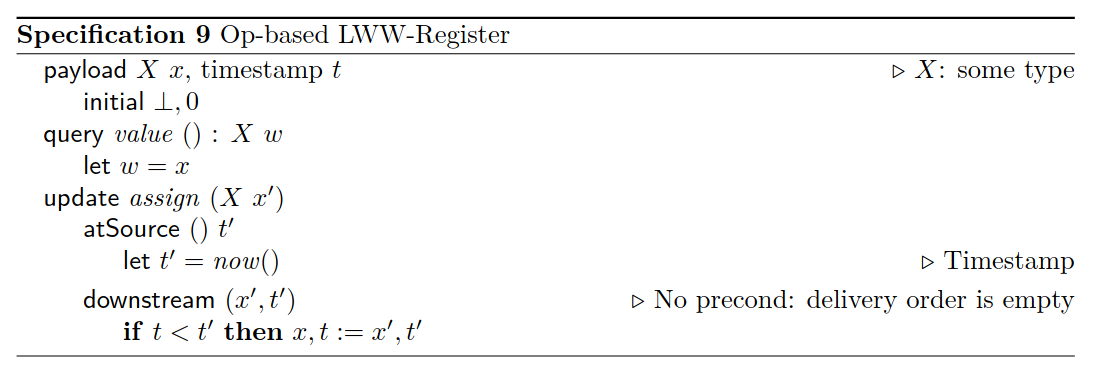
\includegraphics[width=\textwidth]{lww-definition}
    \caption{Last Writer Wins Register}
    \label{fig:lww-def}
\end{figure}

In order to prove that the LWW Register is Strongly Eventually
Consistent, we need to prove that all different concurrent effects
(indicated as ``downstream'' in \cref{fig:lww-def}) commute. We
consider the Since only the value $x$ of the register can be returned
using queries, we consider two states to be equivalent if their values
$x$ and timestamps $t$ are equal.

We started by encoding the state as a value $x$ of any type $X$ and a
timestamp $t$ of type $Int$. In order to encode the \texttt{effect} of
the $assign$ method we need to ensure that the timestamp $t'$ is
unique. In order to achieve that, we need to extend the state with an
additional component $SeenTimestamps$ that contains the set of all
timestamps that have been encountered so far. This auxiliary component
can be used to encode uniqueness as the \texttt{effect}-method
precondition:

\[
t' \not \in SeenTimestamps \wedge t \in SeenTimestamps
\]

\noindent
This ensures that all new timestamps cannot be in the set of seen
timestamps and that the current timestamp is in the set (which is an
invariant). We then specified the effect method postconditions as seen
in its specification. Servois successfully verified that the effect
method commutes with itself.


\subsection{Grow-only Set and Two-Phase Set}

We have encoded the Grow-only Set (GSet) and Two-Phase Set (2PSet)
from \cite{baquero2017pure}. GSets only support adding items, and they
can be useful when logging events where order is unimportant
(e.g. when storing IPs of clients visiting a web-site). 2PSets extend
GSets by supporting removals, but items that have been removed can
never be added again. Their definitions are shown in
\Cref{fig:gset-def,fig:2pset-def}.

\begin{figure}[h]
    \centering
    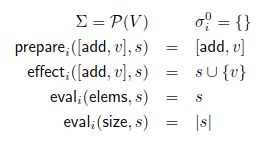
\includegraphics[width=0.4\textwidth]{grow-only-set-definition}
    \caption{Grow-only Set}
    \label{fig:gset-def}
\end{figure}

The state of a GSet is just an originally empty set of values of type
$V$. It's only update function is \texttt{add} which does nothing in
the \texttt{prepare} stage, and then updates the state by inserting
the input element $v$ in the set $s$. The two supported queries are
asking for the elements and the size of the state. The specification
of 2PSet can be seen as a composition of 2 GSets, one for additions
and one for removals. The removals set prohibits items from being
readded to the additions set. 2PSet supports two updating functions,
\texttt{add $v$} and \texttt{remove $v$}. Addition inserts the element
in the addition set only if it doesn't not occur in the removal set,
and removal removes an element from the addition set and adds it in
the removal set. The intuition behind the commutativity of 2PSet is
that removals don't need to happen after an addition to remove the
item, so reversing the order of an addition and a removal of the same
value results in the item being removed.


\begin{figure}[h]
    \centering
    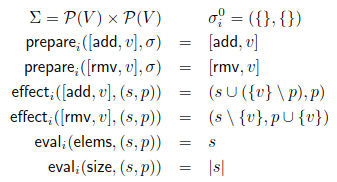
\includegraphics[width=0.5\textwidth]{2pset-definition}
    \caption{Two-Phase Set}
    \label{fig:2pset-def}
\end{figure}

Encoding the two specifications in Servois is mostly straightforward
since all the \texttt{prepare} methods are identity functions without
preconditions. We just encode the result of their effects as
postconditions. Here is an excerpt of the specification of 2PSet,
specifically the state definition and the effect of the \texttt{add}.

\begin{verbatim}
  state:
    - name: Add
      type: (Set V)
    - name: Remove
      type: (Set V)

  methods:
    - name: add
      args:
        - name: v
          type: V
      return:
        - name: result
          type: Bool
      requires: |
        true
      ensures: |
        (and result
             (= Add_new (union (setminus (singleton v) Remove) Add))
             (= Remove_new Remove))
\end{verbatim}

\subsection{Graph CRDTs}

Our final attempt to encode a CRDT was the directed graph specified in Section 5
of \cite{shapiro2011conflict}. It allows for conflict-free queries, additions,
and deletions of nodes and edges. The specification for the directed graph CRDT
can be seen in \Cref{fig:graph-def}. At a high-level, this graph allows for
simultaneous additions and deletions of vertices and edges across replicas.
These updates are reflected as sets representing the change made by each
operation, and periodically these deltas are sent as updates to all other
replicas. The mechanism by which we are able to handle duplicate
insertions/references is by associating every vertex and edge with a unique tag.

\begin{figure}[h]
    \centering
    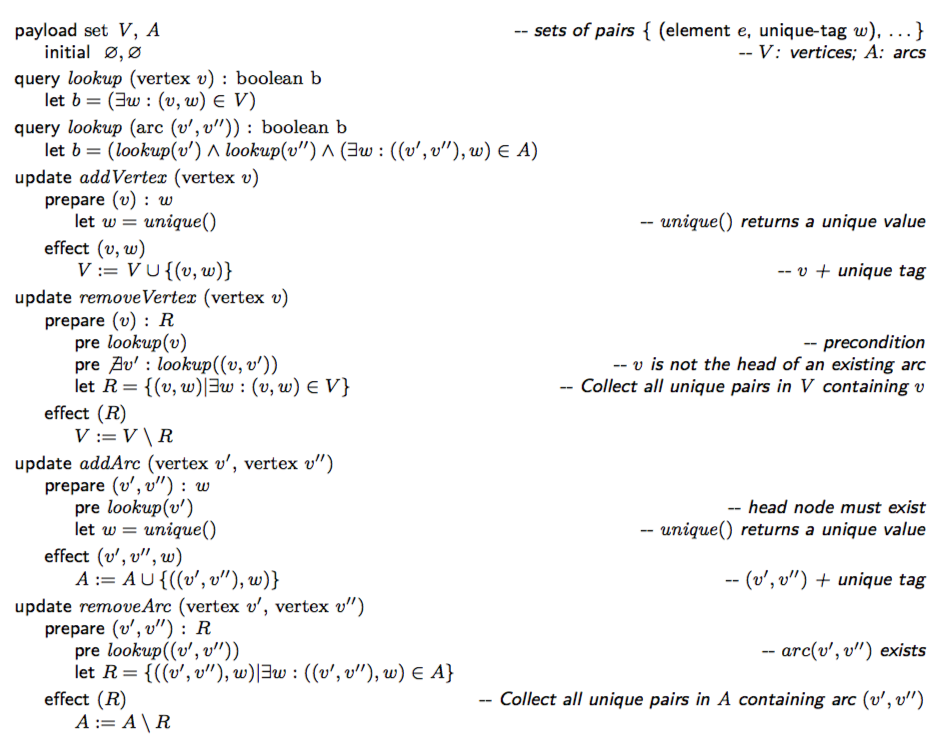
\includegraphics[width=1\textwidth]{directed-graph-def}
    \caption{Op-based Directed Graph Specification}
    \label{fig:graph-def}
\end{figure}


We were able to come up with a straightforward translation of the spec using
CVC4's theory of sets and arrays. However, there were two main issues that
prevented Servois from being able to find commutativity conditions. The
\textit{removeVertex} and \textit{removeArc} (edge) preconditions have an
$\exists$ condition, and CVC4 would immediately return ``unknown'' when queried.
Though we do not know exactly why this occurred, we suspect it is because of the
nested quantification that occurs when introducing an $\exists$ clause in the
specification. Even when we refactored the logic to use a $\forall$, CVC4 still
could not solve the query.

Many of the more complex CRDT specifications contained specifications that
involved quantifiers. It would be interesting to see if these could be
refactored to be quantifier-free. It is important to note that all the example
CRDTs in the Servois paper had quantifier-free encodings. Furthermore, their
method was careful to come up with alternative formulations that avoided
``$\forall\exists$'' quantifier alternation, which they noted would make queries
undecidable \cite{bansal2018servois}.

%% Bibliography
\bibliography{./draft}
\bibliographystyle{plain}



\end{document}
